%%%% 補助スライド
\appendix
\backupbegin

\begin{frame}{}
 補足
\end{frame}

\begin{frame}{クイーングラフ}
 \begin{block}{クイーングラフ}
  $n\times n$のチェス盤について各マスを頂点とし,
  クイーンが移動できるマス同士が辺で結ばれているグラフを
  \structure{クイーングラフ}といい,$Q_n$と表す.
 \end{block}
 \begin{exampleblock}{クイーングラフの例: $Q_3$}
  例として,サイズ$3 \times 3$のチェス盤と
  クイーングラフ$Q_3$の対応関係を下図に示す.
  \begin{figure}[htb]
   \label{ex:queengraph_3}
   \begin{minipage}[b]{0.2\linewidth}
    \centering
    \begin{tikzpicture}
 \draw[gray] (-0.75,-0.75)--(-0.75,0.75);
 \draw[gray] (-0.25,-0.75)--(-0.25,0.75);
 \draw[gray] (0.25,-0.75)--(0.25,0.75);
 \draw[gray] (0.75,-0.75)--(0.75,0.75);
 \draw[gray] (-0.75,-0.75)--(0.75,-0.75);
 \draw[gray] (-0.75,-0.25)--(0.75,-0.25);
 \draw[gray] (-0.75,0.25)--(0.75,0.25);
 \draw[gray] (-0.75,0.75)--(0.75,0.75);
 \draw[red][<->] (0.5,-0.5)--(-0.5,0.5);
 \draw[red][<->] (-0.5,-0.5)--(0.5,0.5);
 \draw[red][<->] (0,-0.5)--(0,0.5);
 \draw[red][<->] (-0.5,0)--(0.5,0);
 \matrix[matrix of nodes,nodes={inner sep=10pt,text width=1cm,
align=center,minimum height=1cm}]{
  &  & \symqueen  \\
  &  & \\
  &  &  \\};
\end{tikzpicture}
   \end{minipage} 
   \begin{minipage}[b]{0.5\linewidth}
    \centering
    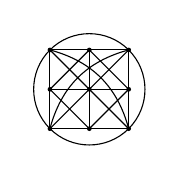
\begin{tikzpicture}
 \draw (-0.5,-0.5)--(-0.5,0.5);
 \draw (0,-0.5)--(0,0.5);
 \draw (0.5,-0.5)--(0.5,0.5);
 \draw (-0.5,-0.5)--(0.5,-0.5);
 \draw (-0.5,0)--(0.5,0);
 \draw (-0.5,0.5)--(0.5,0.5);
 \draw (-0.5,-0.5)--(0.5,0.5);
 \draw (-0.5,0.5)--(0.5,-0.5);
 \draw (-0.5,0)--(0,0.5);
 \draw (-0.5,0)--(0,-0.5);
 \draw (0.5,0)--(0,0.5);
 \draw (0.5,0)--(0,-0.5);
 \draw (-0.5,0.5) to [out=45,in=135] (0.5,0.5);
 \draw (0.5,0.5) to [out=315,in=45] (0.5,-0.5);
 \draw (0.5,-0.5) to [out=225,in=315] (-0.5,-0.5);
 \draw (-0.5,-0.5) to [out=135,in=225] (-0.5,0.5);
 \draw (-0.5,-0.5) to [out=75,in=195] (0.5,0.5);
 \draw (-0.5,0.5) to [out=345,in=105] (0.5,-0.5);
 \foreach \x in {-0.5,0,0.5}
  \foreach \y in {-0.5,0,0.5}
   \fill (\x,\y) circle (0.03);
\end{tikzpicture}
   \end{minipage}
  \end{figure}
 \end{exampleblock}
\end{frame}

\begin{frame}\frametitle{実験結果}
 \begin{itemize}
  \item 各符号化に対して時間内の判定ができた数を比較する.
 \end{itemize}
 \begin{block}{}
  \begin{table}[ht]
   \centering
   \begin{tabular}{c|c|c}
    &SAT &UNSAT \\ \hline
    基本符号化 &3 &3 \\
    改良符号化 &5 &3 \\
    部分和符号化 &{\color{red}7} &3 \\ \hline
   \end{tabular}
  \end{table}
  \begin{itemize}
   \item SATの問題では,\structure{部分和符号化}が
	 最も多くの問題を解きその優位性を確認できた.
   \item UNSATの問題ではどの符号化でも解けた問題数は
	 変わらなかったが,UNSATを導くまでにかかった時間では
	 \structure{部分和符号化}の優位性を確認できた.
  \end{itemize}
 \end{block}
\end{frame}

\backupend